\section{Ablations}
\label{sec:app_ablations}

This section isolates individual components of the LLAMIA pipeline. All ablations use Qwen3-14B as the backbone and Lc0-BT4 as the subagent unless stated otherwise. Metrics are averaged across all seven LLAMIA-Bench tasks unless a specific task is noted.

\subsection{Emergent Collaboration Agency}
\label{sec:abl_agency_strategies}

Verbalization gives the model \emph{answers}: ``best move: e4, eval: +0.3.'' Internalization gives the model \emph{perception}: a 32-token encoding of the engine's full representational state. Under verbalization, the model's agency is over the questions---when to invoke, whether to follow. Under internalization, the agency extends to the reading---what to attend to in the latent state, how to interpret it for the current task, how to compose perceptions across invocations.

\begin{figure}[t]
    \centering
    
\includegraphics[width=\linewidth]{pages/figures/agency_strategy_heatmaps.pdf}
    \caption{\textbf{Collaboration strategy distribution (\%) per task at convergence.}
    Each cell shows the fraction of 500 evaluation episodes classified into that strategy by a GPT-4o judge ($\kappa = 0.78$ vs.\ two human raters; see \cref{sec:app_prompts}).
    \emph{Left} (blue): LLAMIA (latent internalization). \emph{Right} (orange): LLAMIA-Verb (text summaries).
    LLAMIA's dominant strategy shifts with the task: engine-follow for gameplay (65\%), where the engine's top move \emph{is} the answer; consult-then-override for behavior cloning (48\%) and instruction planning (40\%), where the correct action is deliberately suboptimal relative to the engine; and counterfactual query for commentary (40\%), where comparative reasoning across candidate continuations is required.
    LLAMIA-Verb shows no such differentiation---engine-follow dominates every row (62--76\%) because the text interface returns the same compressed summary regardless of how the model queries.
    Quantitatively: LLAMIA's strategy entropy is $H = 1.53$ nats (95\% of maximum $\ln 5$) vs.\ $0.93$ for LLAMIA-Verb (58\%); mean pairwise task-specificity $\overline{\mathrm{JSD}} = 0.12$ vs.\ $0.012$ nats.
    }
    \label{fig:agency_heatmaps}
    \label{sec:abl_agency_strategy_distribution}
    \label{sec:abl_agency_task_specificity}
\end{figure}

Figure~\ref{fig:agency_heatmaps} decomposes this difference. Five collaboration patterns are identified---\emph{engine-follow} (adopt the top recommendation), \emph{consult-then-override} (query then diverge), \emph{counterfactual query} (play a hypothetical move, invoke, undo), \emph{multi-step lookahead} (chain 2--3 counterfactual sequences), and \emph{abstention} (act from language knowledge alone)---and the figure shows how each system allocates across them per task. The internalized model reads the engine differently depending on purpose; the verbalized model treats it as an answering machine. Figure~\ref{fig:agency_task_specificity} traces how both metrics evolve during training.

\begin{figure}[t]
    \centering
    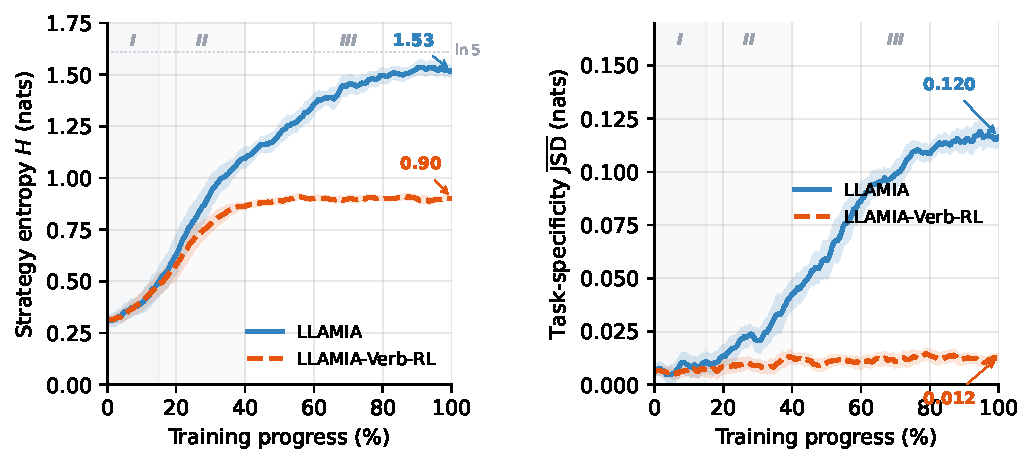
\includegraphics[width=\linewidth]{pages/figures/agency_diversity_training.pdf}
    \caption{\textbf{The integration interface determines what kind of collaborator the model becomes.}
    Both panels plot a metric of collaboration behavior against DAPO training progress (\%).
    Solid blue: LLAMIA (latent internalization). Dashed orange: LLAMIA-Verb (verbalized tool use, same backbone and recipe). Shaded bands: running standard deviation.
    \emph{Left:} Strategy entropy $H$ (nats) over the five collaboration patterns in \cref{fig:agency_heatmaps}. Maximum entropy is $\ln 5 = 1.61$ (dotted line). Through ${\sim}$30\% of training, both systems develop similar diversity ($H \approx 0.75$): the model learns \emph{when} to invoke and \emph{whether} to follow---agency over the questions, available to both interfaces. After ${\sim}$40\%, the curves diverge. LLAMIA's entropy rises to $H = 1.53$ (95\% of maximum) as counterfactual-query and multi-step-lookahead patterns emerge---agency over the reading, available only through the latent channel. LLAMIA-Verb plateaus at $H = 0.93$ (58\%); no new patterns appear because the text response carries the same compressed summary regardless of how the model queries.
    \emph{Right:} Task-specificity ($\overline{\mathrm{JSD}}$, nats) between per-task strategy distributions (\cref{fig:agency_heatmaps}). LLAMIA's strategies diverge across tasks: override dominates behavior cloning (48\%), and counterfactual query dominates commentary (40\%). LLAMIA-Verb's distribution is engine-follow on every task (62--76\%), yielding $\overline{\mathrm{JSD}} = 0.012$---an order of magnitude below LLAMIA's $0.12$. The verbalized model has learned one way to use the engine; the internalized model has learned six.
    }
    \label{fig:agency_task_specificity}
\end{figure}

\subsection{Agent Size and Playing Strength}
\label{sec:app_abl_agent_size_playing_strength}

This ablation asks whether internalization gains are tied to BT4 specifically or generalize across agent architectures and capacities. We draw the agent pool from five additional Lc0 networks spanning roughly 2000--2600\,Elo, covering three architectural families---convolutional SE-ResNets (T72, T78), standard transformers (T80, T82), and big transformers (BT3)---so that architecture is separated from raw capacity. All Elos are measured \emph{without search} (single forward pass, policy-only decoding) via the gauntlet protocol : LLAMIA internalizes the agent's single-forward-pass representation through the LatentBridge, so the no-search rating reflects the information actually available to internalization---tree-search budget is not distilled into the latent state. Table~\ref{tab:lc0_crosscheck} lists the networks, with BT4 included as the primary agent for reference.

\begin{table}[h]
\centering
\setlength{\tabcolsep}{5pt}
\caption{%
  \textbf{Lc0 network pool for the agent-size ablation.}
  Elo is measured without search (policy-only, single forward pass) via the
  gauntlet protocol.
  BT4 is the primary agent used throughout the paper.
}
\label{tab:lc0_crosscheck}
\begin{adjustbox}{max width=\columnwidth}
\renewcommand{\arraystretch}{1.3}
\small
\begin{tabular}{llrr}
\toprule[1.2pt]
\textbf{Network} & \textbf{Architecture} & \textbf{Params}
  & \textbf{Elo (no search)} \\
\midrule
T72   & SE-ResNet, 256$\times$20  & 40M  & 2{,}010 \\
T78   & SE-ResNet, 384$\times$20  & 95M  & 2{,}180 \\
T80   & Transformer, 768$\times$15$\times$24h  & 109M & 2{,}250 \\
T82   & Transformer, 768$\times$15$\times$24h  & 109M & 2{,}292 \\
BT3   & Transformer, 768$\times$15$\times$24h  & 160M & 2{,}510 \\
\midrule
BT4\textsuperscript{$\star$}
      & Transformer, 1024$\times$15$\times$32h & 240M & 2{,}810 \\
\bottomrule[1.2pt]
\end{tabular}
\end{adjustbox}
\end{table}

We replace BT4 (240M params, $\sim$2810\,Elo without search, $\sim$3300 with 1000-node MCTS) with progressively weaker networks from this pool. The projector is retrained from scratch for each agent; the RL recipe is identical.

\begin{table}[h]
\centering
\caption{\textbf{Agent-size ablation.} LLAMIA-14B performance with different Lc0 backends. BC and Commentary are representative tasks; Avg.\ is the unweighted mean across all LLAMIA-Bench tasks. Stronger agents yield monotonically better scores.}
\label{tab:abl_agent_size}
\begin{adjustbox}{max width=\columnwidth}
\renewcommand{\arraystretch}{1.25}
\small
\begin{tabular}{lcccc}
\toprule[1.2pt]
\textbf{Agent} & \textbf{Elo (no search)} & \textbf{BC} & \textbf{Comm.} & \textbf{Avg.} \\
\midrule
T72   & $\sim$2000 & 44 & 52 & 38.7 \\
T80   & $\sim$2200 & 49 & 62 & 46.3 \\
T82   & 2292       & 51 & 66 & 48.9 \\
BT3   & $\sim$2500 & \valgood{53} & \valgood{71} & \valgood{51.7} \\
BT4   & $\sim$2810 & \valbest{56} & \valbest{75} & \valbest{56.9} \\
\bottomrule[1.2pt]
\end{tabular}
\end{adjustbox}
\end{table}

Stronger agents monotonically improve LLAMIA across the representative tasks and the overall average, indicating that the projected representation preserves capability-relevant information. The trend does not rely on BT4 alone: T72 and T80 follow the same ordering on behavior cloning and commentary under the identical training recipe.

\subsubsection{LLM Backbone and Agent Strength}
\label{sec:app_abl_scaling_both_axes}

Figure~\ref{fig:scaling_bars} extends the agent-size ablation to two LLM backbones (4B and 14B) across the same five agents, now spanning both SE-ResNet and Transformer architectures (Table~\ref{tab:lc0_crosscheck}). Performance increases monotonically with both LLM capacity and agent strength on all representative tasks.

The 4B-to-14B improvement is 2.4--3.1$\times$ larger for Transformer-architecture agents (T80, BT3, BT4) than for SE-ResNet agents (T72, T78). The ratio is largest on Interest ($3.1\times$) and Commentary ($2.7\times$), the two tasks most dependent on reading the agent's internal representation, and smallest on Behavior Cloning ($2.4\times$). On Interest, the 4B scores for the strongest SE-ResNet agent (T78, 40) and the weakest Transformer agent (T80, 41) are nearly identical, yet their 14B scores diverge sharply (46 vs.\ 55). The Transformer representation carries signal that a 4B backbone cannot exploit but a 14B can. Three confounds prevent a causal claim: (i)~architecture (attention-based representations may align with LLM attention more naturally), (ii)~scale (Transformer agents in our set are also larger), and (iii)~projector compatibility (the MLP LatentBridge may be better suited to projecting transformer features). Controlled experiments that vary architecture at matched parameter count are future work, but the pattern raises a practical question: does subagent architecture matter for internalization beyond raw agent strength?

\begin{figure}[t]
    \centering
    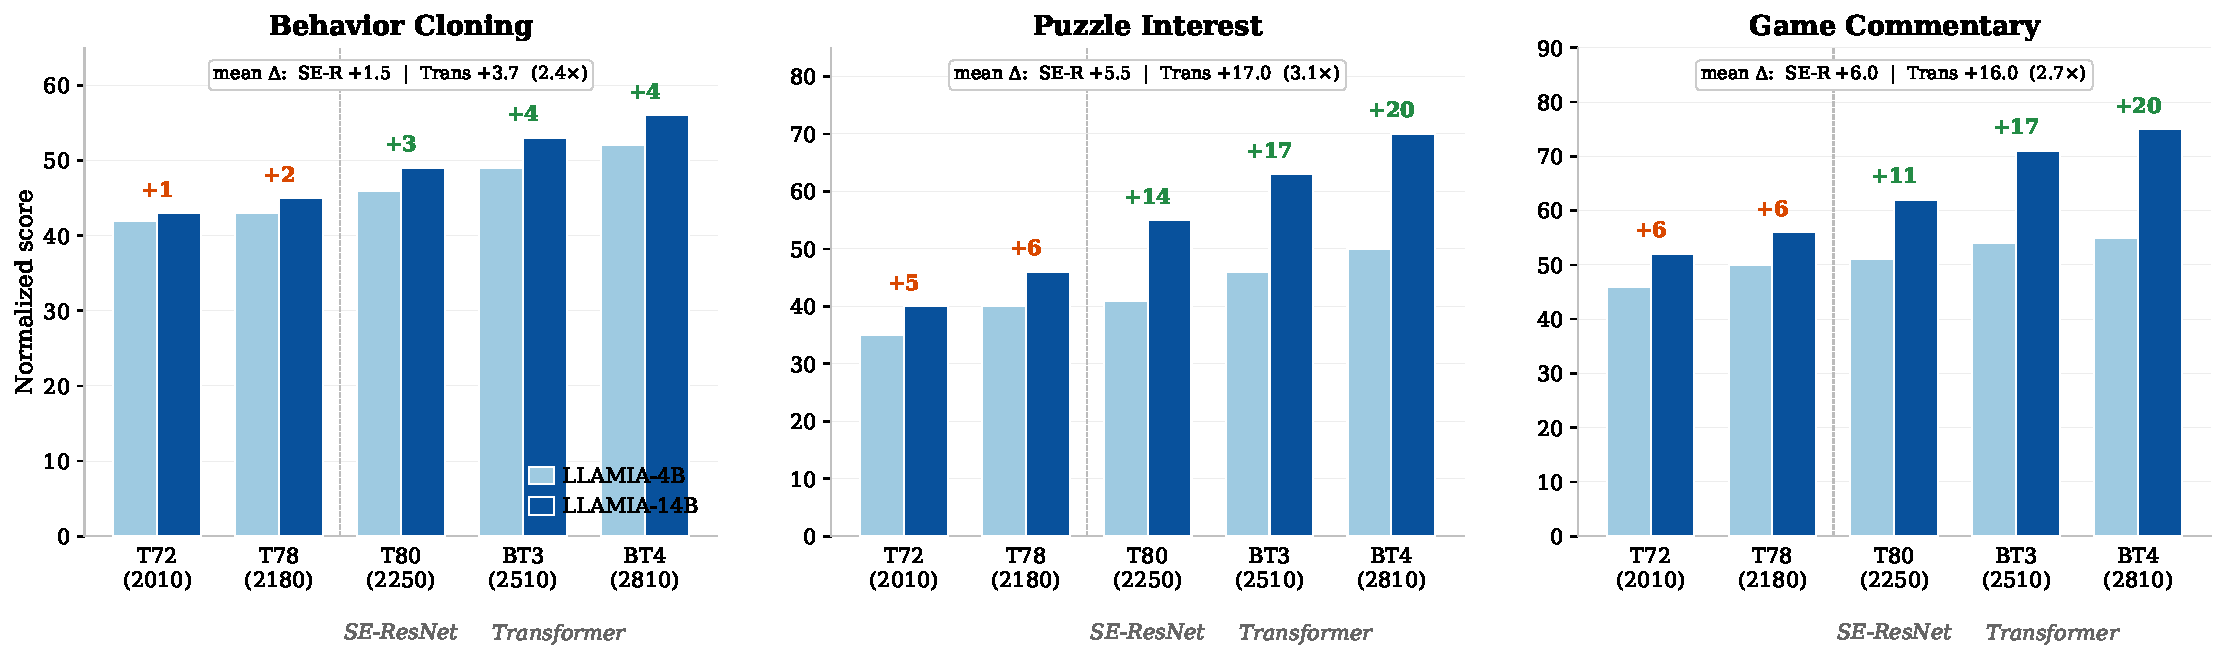
\includegraphics[width=\linewidth]{pages/figures/scaling_bars_1x3.pdf}
    \caption{\textbf{LLM backbone $\times$ agent architecture and strength.}
    Each panel shows one representative LLAMIA-Bench task (Behavior Cloning, Puzzle Interest, Game Commentary).
    $x$-axis: Lc0 agents ordered by architecture family (SE-ResNet \emph{left}, Transformer \emph{right}) and by playing strength (Elo without search, in parentheses).
    Bars: LLAMIA-4B (light blue) and LLAMIA-14B (dark blue).
    Green/brown annotations: the 4B$\to$14B improvement $\Delta$.
    Performance increases with both LLM capacity and agent strength.
    The $\Delta$ is consistently larger for Transformer agents than for SE-ResNet agents, with the effect strongest on representation-intensive tasks (Interest $3.1\times$, Commentary $2.7\times$).
    Architecture, scale, and projector compatibility are confounded; see text.}
    \label{fig:scaling_bars}
\end{figure}

\subsection{Projection Token Count}
\label{sec:app_abl_projection_token_count}
\label{sec:token_ablation}

We vary the number of state tokens $k \in \{4, 8, 16, 32, 64\}$ injected per \texttt{<invoke>} call. Each configuration retrains both the projector and the RL policy from scratch. Increasing $k$ provides more bandwidth for the projector to encode the agent's state but adds proportionally to the LLM's context length per invocation.

\begin{table}[h]
\centering
\caption{\textbf{Projection token count ablation.} LLAMIA-14B with varying $k$. BC and Commentary are representative tasks; Avg.\ is the unweighted mean across all LLAMIA-Bench tasks. Performance saturates at $k{=}32$, which is used throughout.}
\label{tab:abl_tokens}
\begin{adjustbox}{max width=\columnwidth}
\renewcommand{\arraystretch}{1.25}
\small
\begin{tabular}{ccccc}
\toprule[1.2pt]
$k$ & \textbf{BC} & \textbf{Comm.} & \textbf{Avg.} & \textbf{Tokens/episode} \\
\midrule
4   & 48 & 58 & 45.1 & 680 \\
8   & 51 & 65 & 49.7 & 720 \\
16  & \valgood{54} & \valgood{73} & 54.9 & 790 \\
32  & \valbest{56} & \valbest{75} & \valbest{56.9} & 920 \\
64  & 56 & 75 & \valgood{56.7} & 1180 \\
\bottomrule[1.2pt]
\end{tabular}
\end{adjustbox}
\end{table}

Performance increases monotonically from $k{=}4$ to $k{=}32$ and changes little at $k{=}64$. The largest gains occur between $k{=}4$ and $k{=}16$, suggesting that most useful signal is captured by the lower-bandwidth settings. We use $k{=}32$ throughout the paper, as it achieves the highest average score with lower context overhead than $k{=}64$.
